\subsection{sketch.js}
Cree un archivo sketch.js y evalue sus resultados.
\begin{lstlisting}[language=C++,
                   directivestyle={\color{black}}
                   emph={int,char,double,float,unsigned},
                   emphstyle={\color{blue}}
                  ]
function setup() {
  var width = 250;
  var height = 200;
  var canvas = createCanvas(width, height);
  background(0);
  for (var x = 0; x < width; x += width / 10) {
    for (var y = 0; y < height; y += height / 5) {
      stroke(125, 125, 125);
      strokeWeight(1);
      line(x, 0, x, height);
      line(0, y, width, y);
    }
  }
  var data = [];
  for (let i = 0; i < 12; i++) {
    var x = Math.floor(Math.random() * height);
    var y = Math.floor(Math.random() * height);
    data.push([x, y]);
    fill(255, 255, 255);
    circle(x, height - y, 7);
    textSize(8);
    text(x + ',' + y, x + 5, height - y);
    
  }
  var root = build_kdtree(data);
  console.log(root);
}
\end{lstlisting}
\begin{figure}[H]
  \centering
  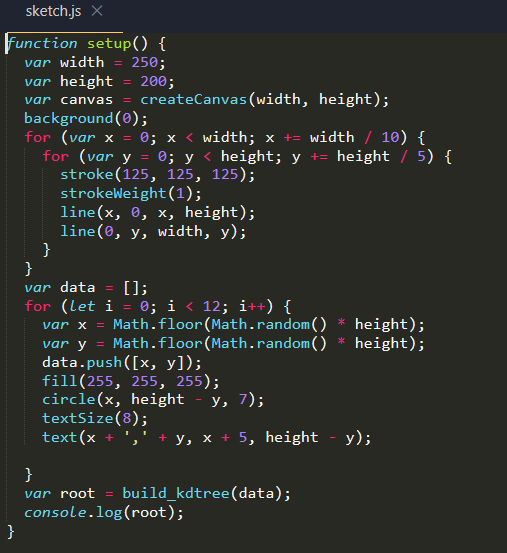
\includegraphics[width=0.5\textwidth]{images/tres.PNG}
  \caption{sketch.js}
  \label{fig:act-2}
\end{figure}

\begin{figure}[H]
  \centering
  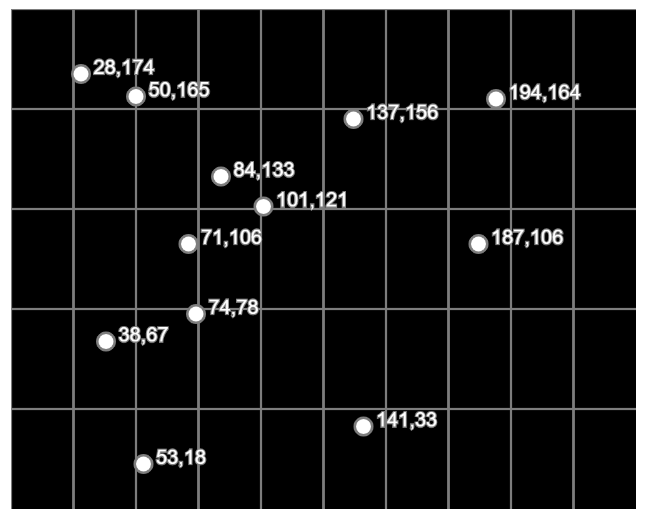
\includegraphics[width=0.6\textwidth]{images/dos.PNG}
  \caption{Puntos generados aleatoriamente}
  \label{fig:act-3}
\end{figure}

\begin{figure}[H]
  \centering
  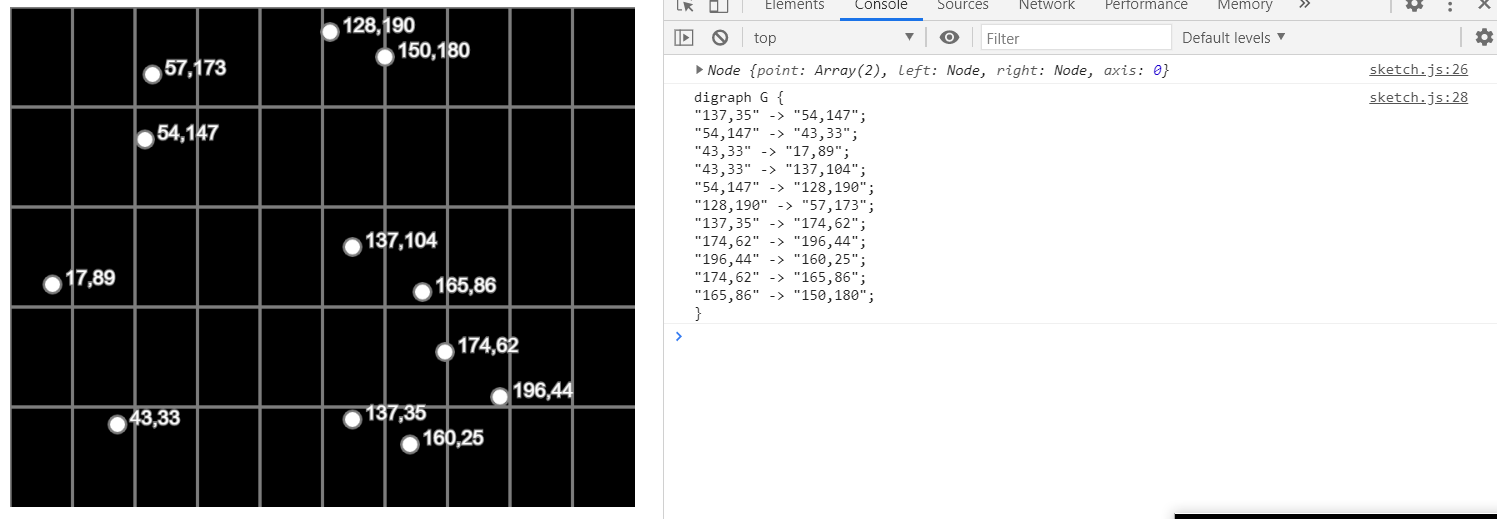
\includegraphics[width=1.1\textwidth]{images/cuatro.PNG}
  \caption{Formato dot en la consola}
  \label{fig:act-4}
\end{figure}
